\section{Kadek Diva Krishna Murti}
{\Large \textbf{Pemahaman Teori}}
\subsection{Soal No. 1}
Apa itu fungsi device manager di windows dan folder /dev di linux?

\hfill \break
Device manager merupakan perangkat lunak untuk menampilkan seluruh perangkat keras yang di-inisialisasi atau dikenali oleh sistem operasi Windows. Device Manager membantu dalam mengelola atau me-manage semua perangkat keras yang terpasang dan terdeteksi dalam sistem Windows. Perangkat keras tersebut bisa berupa harddisk, kartu VGA, sound, keyboard, perangkat USB dan lain-lainnya.

\hfill \break
Fungsi device manager antara lain :
\begin{enumerate}
	\item Menunjukkan status mengenai suatu perangkat keras.
	\item Menunjukkan informasi detail mengenai suatu perangkat keras.
	\item Mengelola driver perangkat keras.
	\item Menonaktifkan dan mengaktifkan perangkat keras.
	\item Mengidentifikasi konflik antar perangkat keras.
	\item Memberitahukan terjadinya masalah pada perangkat keras.
\end{enumerate}

\hfill \break
Folder /dev merupakan representasi dari drive yang terhubung ke sistem operasi Linux dan oleh sistem dianggap sebagai file-file direktori. Biasanya sering ditampilkan direktori seperti /dev/sda1 yang mewakili Drive SATA pertama dalam sistem.

\subsection{Soal No. 2}
Jelaskan langkah-langkah instalasi driver dari arduino!

\hfill \break
Berikut ini adalah langkah-langkah instalasi driver dari Arduino UNO di Windows:

\begin{enumerate}
	\item Pertama pastikan Arduino IDE telah terinstall.
	\item Lalu hubungkan port USB Arduino Uno ke port USB PC.
	\item Kemudian PC anda akan mendeteksi perangkat baru yang terpasang dan akan muncul pop seperti ini.
	\begin{figure}[H]
		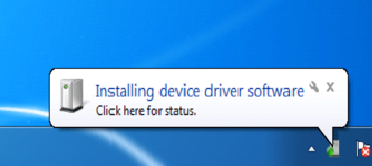
\includegraphics[width=10cm]{figures/5/1174006/Teori/1.png}
		\centering
	\end{figure}
	\item Karena Arduino Uno baru pertama kali terpasang, maka akan muncul pop up error seperti ini.
	\begin{figure}[H]
		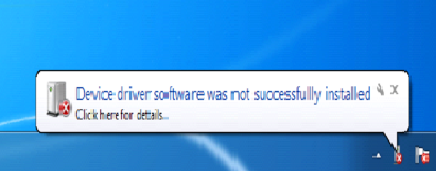
\includegraphics[width=10cm]{figures/5/1174006/Teori/2.png}
		\centering
	\end{figure}
	\item Buka ''Start'' lalu cari Device Manager, kemudian klik ''Device Manager''.
	\begin{figure}[H]
		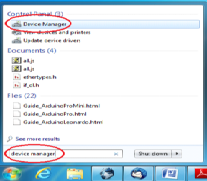
\includegraphics[width=10cm]{figures/5/1174006/Teori/3.png}
		\centering
	\end{figure}
	\item Setelah Device Manager terbuka, silahkan cari ''Unknown Device'' yang berada di Other Device.
	\begin{figure}[H]
		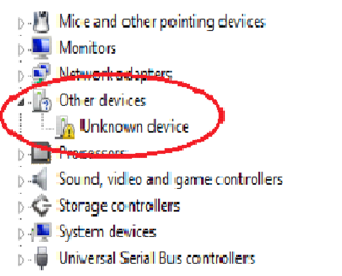
\includegraphics[width=10cm]{figures/5/1174006/Teori/4.png}
		\centering
	\end{figure}
	\item Kemudian klik kanan pada ''Unknown Device'', lalu pilih ''Update Driver Software''.
	\begin{figure}[H]
		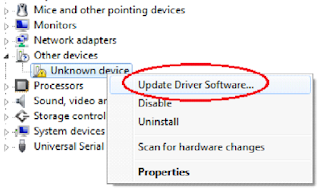
\includegraphics[width=10cm]{figures/5/1174006/Teori/5.png}
		\centering
	\end{figure}
	\item Setelah itu muncul window baru, lalu pilih ''Browse my computer for driver software''.
	\begin{figure}[H]
		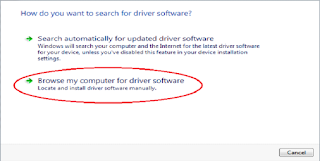
\includegraphics[width=10cm]{figures/5/1174006/Teori/6.png}
		\centering
	\end{figure}
	\item Lalu cari folder yang terinstall Arduino IDE dengan mengklik browse. Kemudian klik ''Next''.
	\begin{figure}[H]
		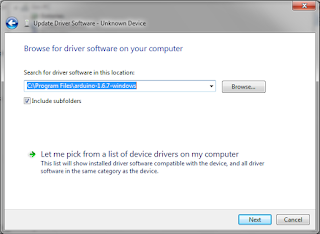
\includegraphics[width=10cm]{figures/5/1174006/Teori/7.png}
		\centering
	\end{figure}
	\item Windows akan mencari dan menginstall driver yang berada pada folder tersebut.
	\begin{figure}[H]
		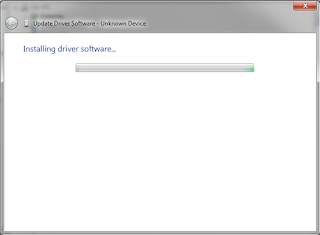
\includegraphics[width=10cm]{figures/5/1174006/Teori/8.png}
		\centering
	\end{figure}
	\item Setelah itu akan muncul window, lalu klik ''Install''.
	\begin{figure}[H]
		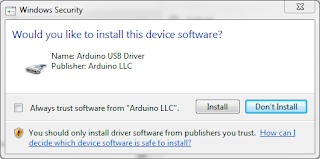
\includegraphics[width=10cm]{figures/5/1174006/Teori/9.png}
		\centering
	\end{figure}
	\item Jika berhasil terinstal maka akan muncul window seperti ini.
	\begin{figure}[H]
		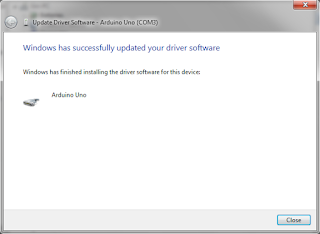
\includegraphics[width=10cm]{figures/5/1174006/Teori/10.png}
		\centering
	\end{figure}
\end{enumerate}

\subsection{Soal No. 3}
Jelaskan bagaimana cara membaca baudrate dan port dari komputer yang sudah terinstall driver!

\hfill \break
\textbf{Membaca Baudrate dari Komputer}
\begin{enumerate}
	\item Pertama buka ''Start''. Cari ''Device Manager'', lalu klik.
	\begin{figure}[H]
		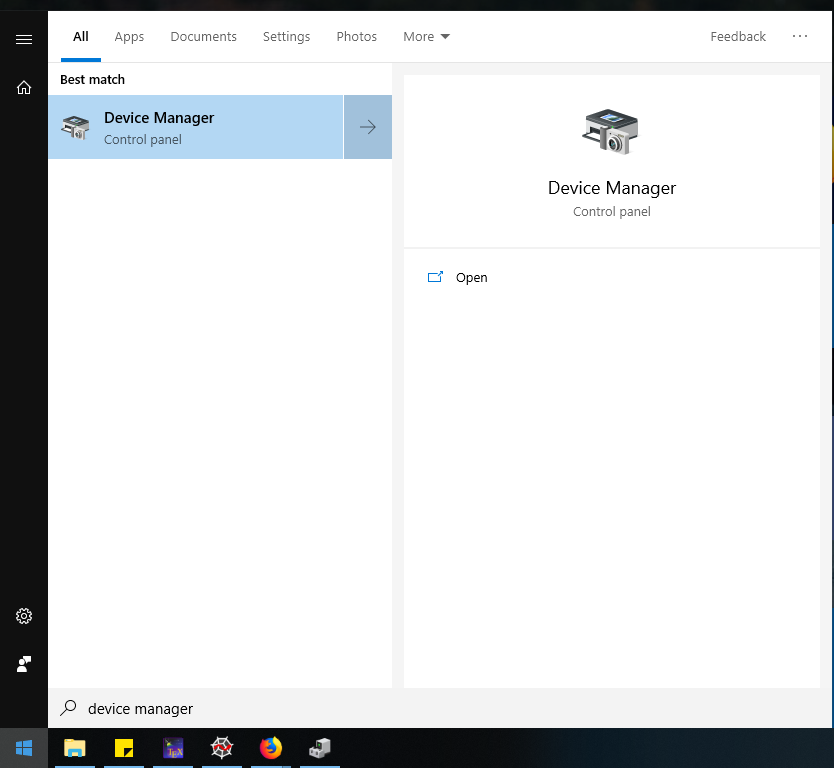
\includegraphics[width=10cm]{figures/5/1174006/Teori/d1.png}
		\centering
	\end{figure}
	
	\item Kemudian pilih ''Ports (COM \& LPT)''.
	\begin{figure}[H]
		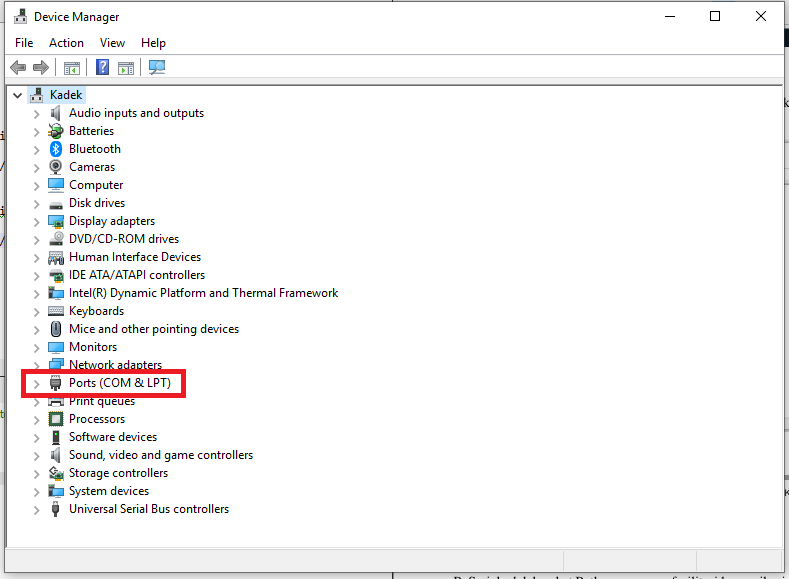
\includegraphics[width=10cm]{figures/5/1174006/Teori/d3.png}
		\centering
	\end{figure}
	
	\item Klik dua kali pada COM yang terhubung.
	\begin{figure}[H]
		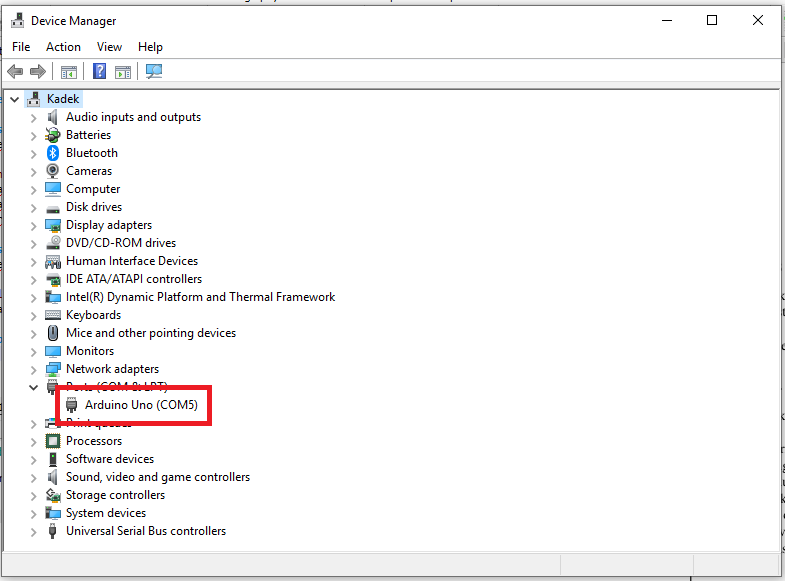
\includegraphics[width=10cm]{figures/5/1174006/Teori/d2.png}
		\centering
	\end{figure}

	\item Pilih tab ''Port Settings'', lalu lihat di ''Bit per second''.
	\begin{figure}[H]
		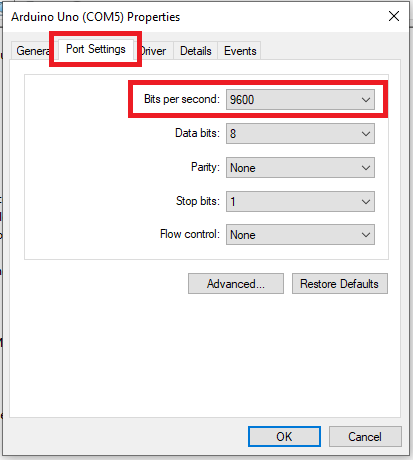
\includegraphics[width=8cm]{figures/5/1174006/Teori/d4.png}
		\centering
	\end{figure}
\end{enumerate}


\hfill \break
\textbf{Membaca Port dari Komputer}

\begin{enumerate}
	\item Pertama buka ''Start''. Cari ''Device Manager'', lalu klik.
	\begin{figure}[H]
		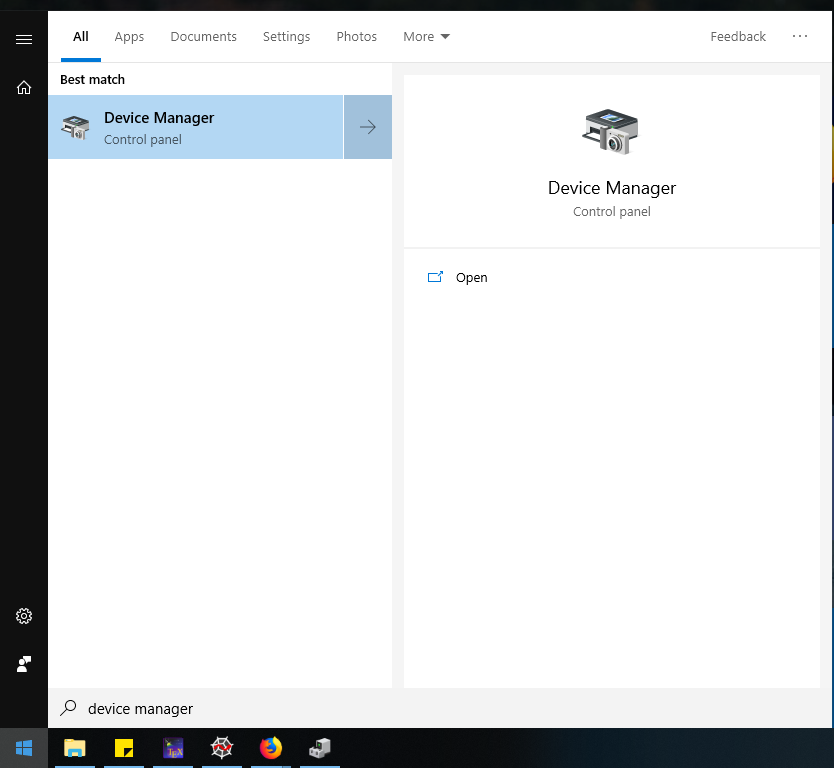
\includegraphics[width=10cm]{figures/5/1174006/Teori/d1.png}
		\centering
	\end{figure}

	\item Kemudian pilih ''Ports (COM \& LPT)''.
	\begin{figure}[H]
		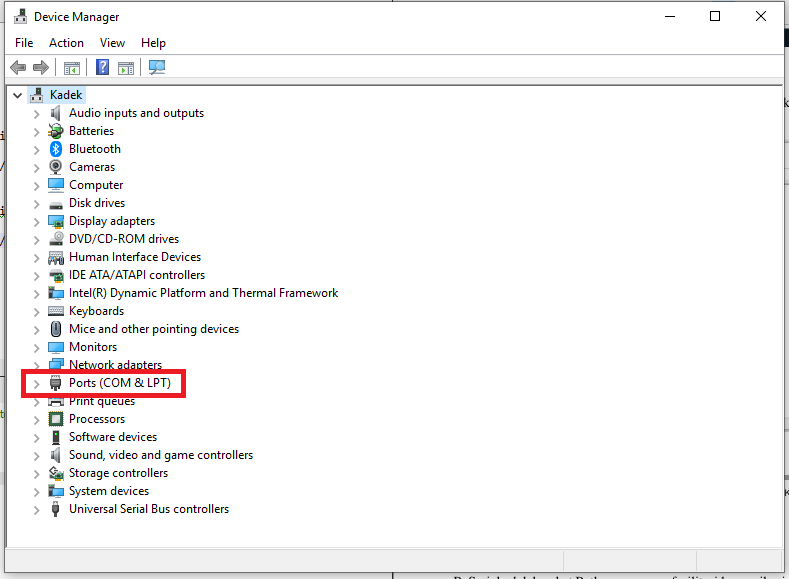
\includegraphics[width=10cm]{figures/5/1174006/Teori/d3.png}
		\centering
	\end{figure}

	\item Port dari Arduino telah terbaca oleh PC.
	\begin{figure}[H]
		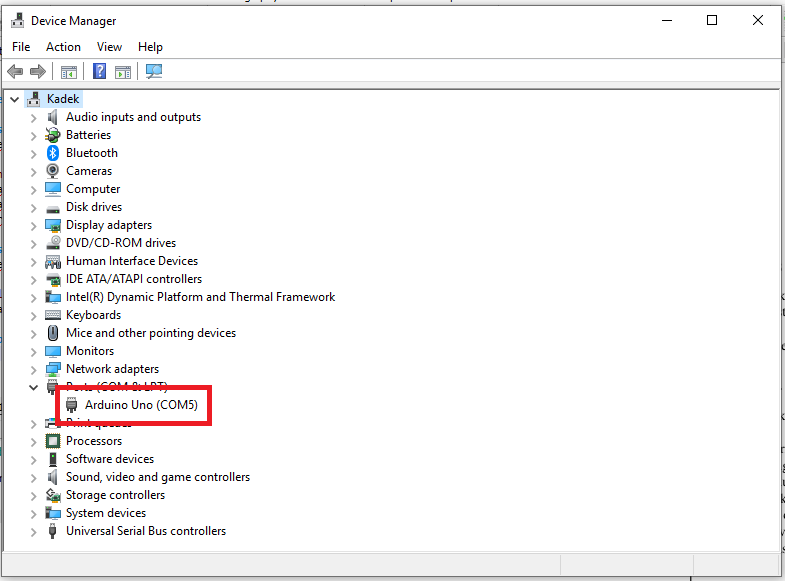
\includegraphics[width=10cm]{figures/5/1174006/Teori/d2.png}
		\centering
	\end{figure}
\end{enumerate}



\subsection{Soal No. 4}
Jelaskan sejarah library pyserial!

\hfill \break
PySerial adalah paket Python yang menfasilitasi komunikasi serial antara PC dengan perangkat keras eksternal. PySerial menyediakan antarmuka untuk berkomunikasi melalui protokol komunikasi serial. Komunikasi serial adalah salah satu protokol komunikasi komputer tertua. Protokol komunikasi serial mendahului spesifikasi USB yang digunakan oleh komputer dan perangkat keras lain seperti mouse, keyboard, dan webcam. USB adalah singkatan dari Universal Serial Bus. USB dan dibangun di atas dan memperluas antarmuka komunikasi serial asli.

\subsection{Soal No. 5}
Jelaskan fungsi-fungsi apa saja yang dipakai dari library pyserial!

\hfill \break
Fungsi-fungsi yang dipakai dari library PySerial, yaitu:
\begin{enumerate}
	\item Serial - fungsi ini untuk membuka port serial.
	\item write(data) - fungsi ini menulis data lewat port serial.
	\item readline() - fungsi ini membaca sebuah string dari port serial.
	\item read(size) - fungsi ini untuk membaca jumlah byte dari port serial.
	\item close() - fungsi ini untuk menutup port serial.
\end{enumerate}

\subsection{Soal No. 6}
Jelaskan kenapa butuh perulangan dan tidak butuh perulangan dalam membaca serial!

\hfill \break
Pada saat membaca serial di Arduino diperlukan perulangan agar bisa membaca data secara berulang kali sehingga data yang muncul banyak. Sedangkan apabila tidak membutuhkan perulangan maka Arduino hanya akan membaca data sekali saja.

\subsection{Soal No. 7}
Jelaskan bagaimana cara membuat fungsi yang mengunakan pyserial!

\lstinputlisting[caption = Fungsi yang menggunakan pyserial., firstline=1, lastline=7]{src/5/1174006/Teori/1174006.py}

\begin{figure}[H]
	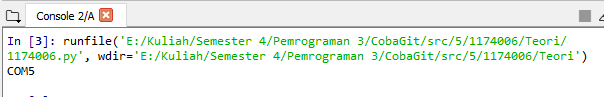
\includegraphics[width=10cm]{figures/5/1174006/Teori/hasil.png}
	\centering
	\caption{Hasil pembuatan fungsi pyserial.}
\end{figure}

\subsection{Cek Plagiat}
\begin{figure}[H]
	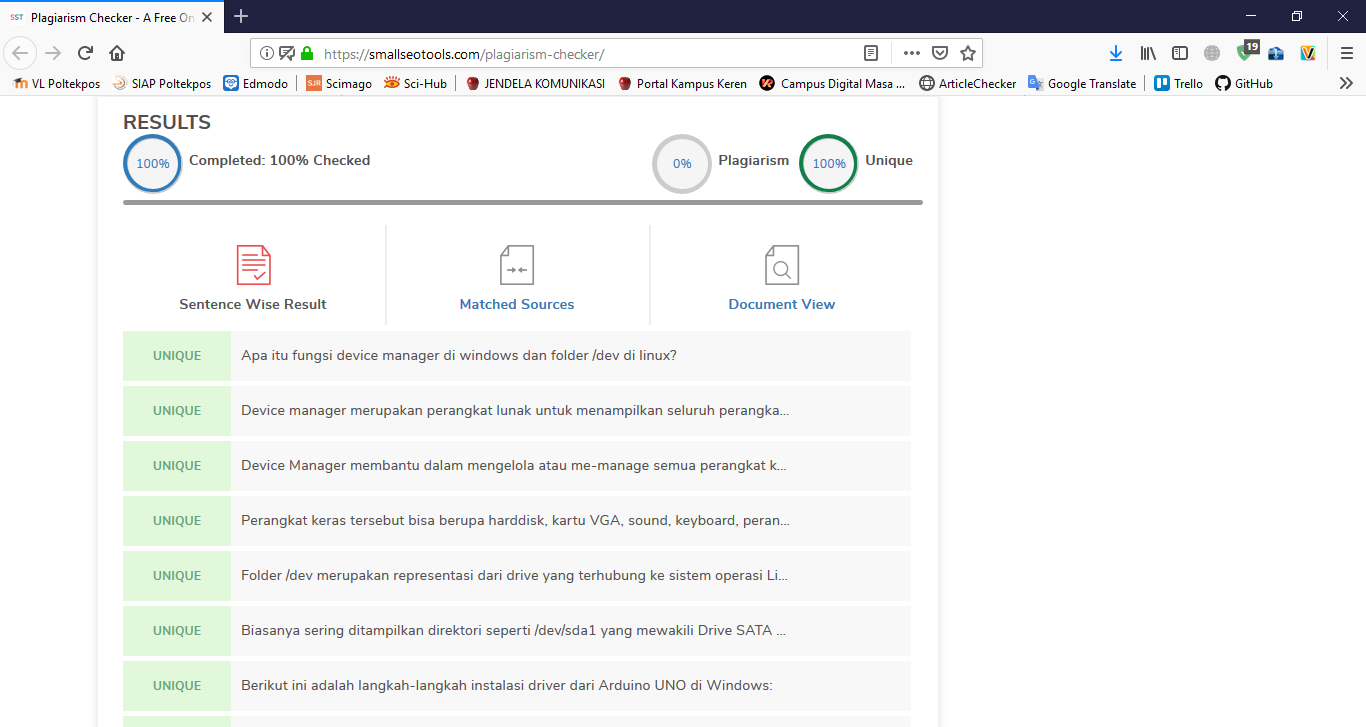
\includegraphics[width=10cm]{figures/5/1174006/Teori/plagiat.png}
	\centering
	\caption{Hasil cek plagiat.}
\end{figure}

\subsection{Kode Program}
\begin{figure}[H]
	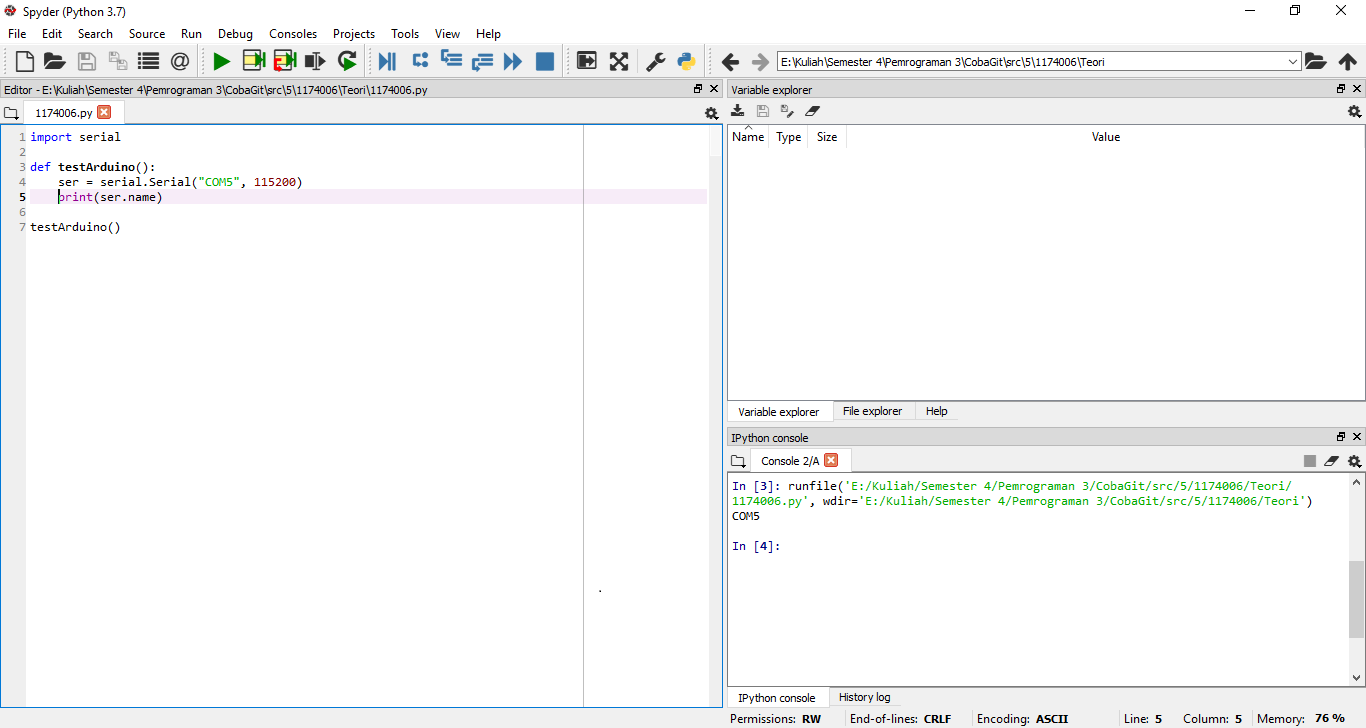
\includegraphics[width=10cm]{figures/5/1174006/Teori/kodeprogram.png}
	\centering
	\caption{Kode program file 1174006.py.}
\end{figure}

%%%%%%%%%%%%%%%%%%%%%%%%%%%%%%%%%%%%%%%%%%%%%%%%%%%%%%%%%%%%%%%%%%%%%%%%%%%%%%%%%%%%%

\section{Muhammad Tomy Nur Maulidy}
{\Large \textbf{Pemahaman Teori}}
\subsection{Soal No. 1}
Apa itu fungsi device manager di windows dan folder /dev di linux?

\hfill \break
Fungsi device manager antara lain :
\begin{enumerate}
	\item Menunjukkan status suatu hardware.
	\item Menunjukkan informasi detil suatu hardware.
	\item Mengelola driver hardware
	\item Disable dan Enable hardware
	\item Mengidentifikasi konflik antar perangkat keras.
\end{enumerate}

\hfill \break
Folder /dev berisi file device, baik device blok maupun device karakter. Di dalamnya setodaknya ada file biner yang beernama MAKEDEV untuk membuat device secara manual.

\subsection{Soal No. 2}
Jelaskan langkah-langkah instalasi driver dari arduino!

\hfill \break
Berikut ini adalah langkah-langkah instalasi driver dari Arduino UNO di Windows:

\begin{enumerate}
	\item Hubungkan sistem minimun Arduino Uno ke komputer dengan kabel USB type B (kabel Printer).
	\item Lalu pada bagian kanan didesktop PC anda, akan muncul popup “Installing device driver software”.
	\item SIstem operasi Windows tidak menyediakan driver untuk Arduino Uno.
	\item Buka Device Manager, caranya pada bagian Search Program and Files lalu ketikkan “device manager” (tanpa tanda petik). Kemudian bagian Control Panel akan muncul halaman Device Manager, selanjutnya klik untuk menjalankan.
	\item Cari yang bernama Unknown device yang berada pada bagian Other device, biasanya ada tanda seru berwarna kuning, itu disebabkan karena penginstallan tidak berjalan dengan sempurna.
	\item Klik kanan pada “Unknown device” kemudian pilih Update Driver Software.
	\item Pilih Browse my computer for driver software.
	\item Arahkan lokasi folder ke folder ..arduino-1.0.5 drivers. Pastikan check-box lalu centang include subfolders. Klik Next untuk melanjutkan instalasi driver.
	\item Kemudian lanjutkan dengan mengklik Install pada tampilan Windows Security.
	\item Jika instalasi driver berhasil maka akan muncul Windows has successfully updated your driver software.
	\item Perhatikan dan ingat nama COM Arduino Uno, karena nama COM ini yang akan digunakan untuk meng-upload program nantinya.
\end{enumerate}

\subsection{Soal No. 3}
Jelaskan bagaimana cara membaca baudrate dan port dari komputer yang sudah terinstall driver!

\hfill \break
\textbf{Membaca Port dari Komputer}

\begin{enumerate}
	\item Hubungkan modul TX-RX serial dengan komputer melalui serial port menggunakan DB9 cable extension.
	\item Buka Hyper Terminal dengan menekan start kemudian All progams lalu Accessories kemudian Communications lalu Hyper Terminal.
	\item Ketik nama untuk Connection Description, misal coba, kemudian tekan OK.
	\item Pada Connect to, pilihlah COM port yang dipakai di Connect using, kemudian tekan OK.
	\item Masukkan nilai-nilai port settingnya, sesuai dengan DCE-nya. Kemudian tekan OK.
\end{enumerate}



\subsection{Soal No. 4}
Jelaskan sejarah library pyserial!

\hfill \break
PySerial adalah library/modul Python siap-pakai dan gratis yang dibuat untuk memudahkan kita dalam membuat program komunikasi data serial RS232 dalam bahasa Python.
Jika modul USB-2REL dapat kita kontrol dengan mudah menggunakan Python dan PyUSB (lihat pembahasannya di sini dan di sini), maka modul SER-2REL juga dapat kita kontrol dengan mudah menggunakan Python dengan bantuan modul PySerial.

\subsection{Soal No. 5}
Jelaskan fungsi-fungsi apa saja yang dipakai dari library pyserial!

\hfill \break
Fungsi-fungsi yang dipakai dari library PySerial, yaitu:
\begin{enumerate}
	\item Serial - fungsi ini untuk membuka port serial.
	\item write(data) - fungsi ini menulis data lewat port serial.
	\item readline() - fungsi ini membaca sebuah string dari port serial.
	\item read(size) - fungsi ini untuk membaca jumlah byte dari port serial.
	\item close() - fungsi ini untuk menutup port serial.
\end{enumerate}

\subsection{Soal No. 6}
Jelaskan kenapa butuh perulangan dan tidak butuh perulangan dalam membaca serial!

\hfill \break
Pada saat membaca serial di Arduino diperlukan perulangan agar bisa membaca data secara berulang kali sehingga data yang muncul banyak. Sedangkan apabila tidak membutuhkan perulangan maka Arduino hanya akan membaca data sekali saja.

\subsection{Soal No. 7}
Jelaskan bagaimana cara membuat fungsi yang mengunakan pyserial!

\hfill \break
Fungsi yang berada pada Python, dibuat dengan nama kata kunci def kemudian diikuti dengan nama fungsinya pada pyhton.
Seperti halnya dengan blok kode yang lain, kita juga harus memberikan identasi untuk menuliskan isi fungsi.

\subsection{Cek Plagiat}
\begin{figure}[H]
	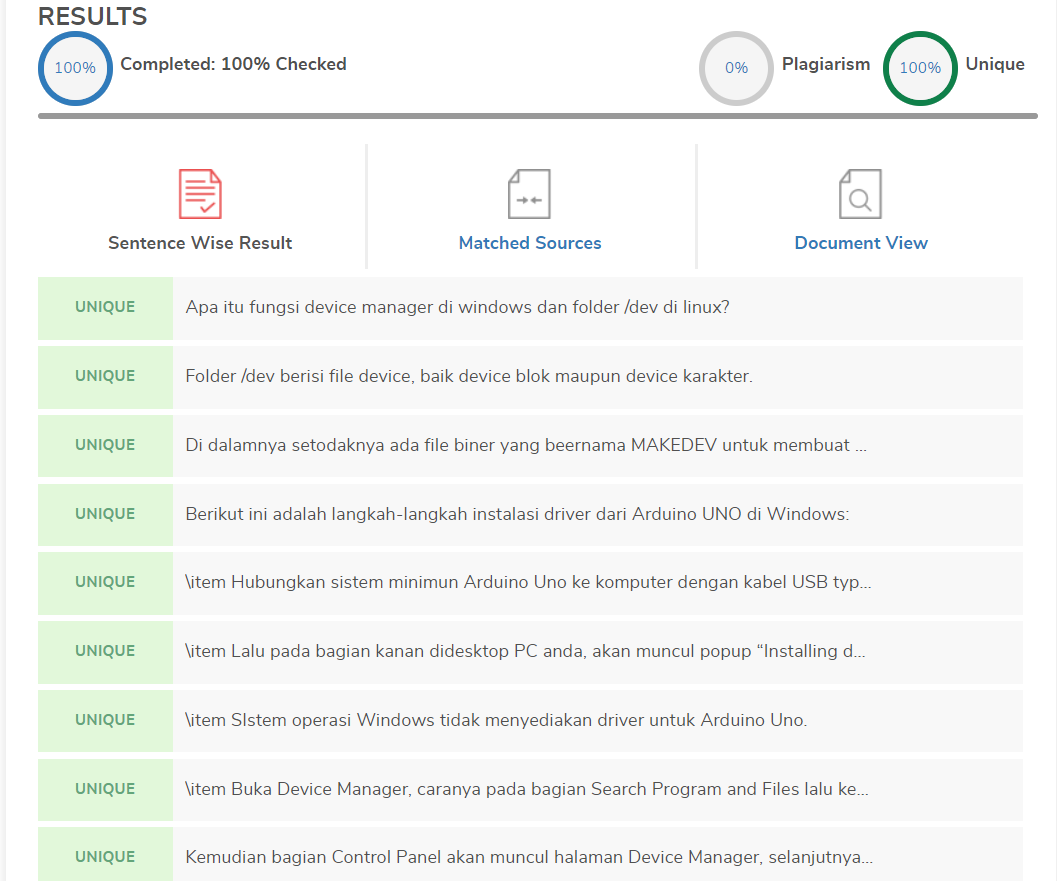
\includegraphics[width=10cm]{figures/5/1174031/Teori/Plagiat.png}
	\centering
	\caption{Hasil cek plagiat.}
\end{figure}
%%%%%%%%%%%%%%%%%%%%%%%%%%%%%%%%%%%%%%%%%%%%%%%%%%%%%%%%%%%%%%%%%5
\section{Damara Benedikta}
\subsection{Apa itu fungsi device manager di windows dan folder /dev di linux}
Windows
Device Manager merupakan Panel Kontrol dalam sistem operasi Microsoft Windows. Ini memungkinkan pengguna untuk melihat dan mengontrol perangkat keras yang terpasang pada komputer. Ketika beberapa bagian perangkat keras tidak berfungsi, perangkat keras yang terkait akan disorot oleh pengguna. Daftar perangkat keras dapat disortir berdasarkan berbagai kriteria.

Untuk setiap perangkat, pengguna dapat:
\begin{itemize}
     \item Menyediakan driver perangkat sesuai dengan Model Driver Windows
     \item Aktifkan atau nonaktifkan perangkat
     \item  Beri tahu Windows untuk mengabaikan perangkat yang tidak berfungsi
     \item Lihat sifat teknis lainnya
\end{itemize}
Device Manager diperkenalkan dengan Windows 95 dan kemudian ditambahkan ke Windows 2000. Dalam versi berbasis NT, ini dimasukkan sebagai snap-in Konsol Manajemen Microsoft.

Linux
/ dev adalah lokasi file khusus atau perangkat. Ini adalah direktori yang sangat menarik yang menyoroti satu aspek penting dari sistem file Linux - semuanya adalah file atau direktori. yang fungsinya untuk menyimpan sebuah konfigurasi device ataupun hardware dari system

\subsection{langkah-langkah instalasi driver dari arduino}
Hubungkan sistem minimun Arduino Uno dan komputer dengan kabel USB type B
Kemudian pada bagian kanan didesktop PC anda, akan muncul popup “Installing device driver software. Pada sIstem operasi Windows tidak tersedia driver untuk Arduino Uno kemudian proses instalasinya dilakukan secara manual.
Yang pertama kalian buka terlebih dahulu Device Managernya, dengan cara pada bagian Search Program and Files kemudian ketikkan “device manager” (tanpa tanda petik), Pada bagian Control Panel akan muncul Device Manager, klik untuk menjalankannya.
Setelah itu kalian cari Unknown device pada bagian Other device, yang biasanya terdapat tanda seru berwarna kuning, itu disebabkan karena penginstallan tidak berjalan dengan sempurna
Selanjutnya Klik kanan pada “Unknown device” kemudian pilihlah Update Driver Software.
Pilihlah Browse my computer for driver software.
Arahkan lokasi folder ke folder."\"arduino-1.0.5"\"drivers. Pastikan check-box kemudian centang include subfolders. Kemudian Klik Next untuk melanjutkan instalasi driver.
Setelah itu  lanjutkan dengan mengklik Install pada tampilan Windows Security.
Jika instalasi driver telah berhasil maka akan muncul Windows has successfully updated your driver software.
Perhatikan dan ingat nama COM Arduino Uno, karena nama COM ini yang akan digunakan untuk meng-upload program nantinya.

\subsection{Jelaskan bagaimana cara membaca baudrate dan port dari komputer yang sudah terinstal driver}
Berikut ini merupakan cara membaca baudrate dan port dari komputer yang sudah terinstal driver :
\begin{itemize}
	\item Sambungkan port USB arduino dengan port USB pc
	\item Kemudian buka software arduino pada pc
	\item Setelah itu, pilih tipe arduino yang digunakan
	\item Kemudian memilih serial port yang aktif  
	\item Selanjutnya untuk memasukkan program pada arduino, klik tombol upload
	\item Setelah proses upload selesai, buka fitur serial monitor
	\item Lalu sesuaikan Baudrate pada serial monitor dengan Baudrate yang terdapat pada program
\end{itemize}

\subsection{Jelaskan sejarah library pyserial}
Pyserial berguna untuk merangkum akses untuk port serial. Pyserial menyediakan backends untuk Python yang berjalan di Windows, Linux, BSD (mungkin sistem yang mendukung POSIX), Jython dan IronPython (.NET dan Mono). Modul bernama "serial" secara otomatis memilih backend yang sesuai. Antarmuka berbasis kelas yang sama pada semua platform yang didukung.
Akses ke pengaturan port melalui properti Python.
Dukungan untuk berbagai ukuran byte, bit stop, paritas dan kontrol aliran dengan RTS / CTS dan / atau Xon / Xoff.
Bekerja dengan atau tanpa menerima batas waktu.
File seperti API dengan "read" dan "write" ("readline" dll. Juga didukung).
File-file dalam paket ini adalah 100 persen Python murni.
Port diatur untuk transmisi biner. Tidak ada stripping byte NULL, terjemahan CR-LF dll. (Yang berkali-kali diaktifkan untuk POSIX.) Ini membuat modul ini bermanfaat secara universal.
Kompatibel dengan pustaka io (Python 2.6+)

\subsection{Jelaskan fungsi-fungsi apa saja yang dipakai dari library pyserial}
Serial – fungsi ini untuk membuka port serial
Write(data) – untuk menulis data lewat port serial
Readline() – untuk membaca string dari port serial
Read(size) – untuk membaca jumlah byte dari port serial
Close() – ini untuk menutup port serial 

\subsection{Jelaskan kenapa butuh perulangan dalam tidak butuh perulangan dalam membaca serial}
Perualangan dalam bahasa pemrograman berfungsi menyuruh komputer melakukan sesuatu secara berulang-ulang. Terdapat dua jenis perualangan dalam bahasa pemrograman python, yaitu perulangan dengan for dan while.
Perulangan for disebut counted loop (perulangan yang terhitung), sementara perulangan while disebut uncounted loop (perulangan yang tak terhitung). Perbedaan yang terlihat adalah pada perulangan for digunakan untuk mengulangi kode yang sudah diketahui banyak perulangannya. Sedangkan perulangan while digunakan pada perulangan yang memiliki syarat dan tidak tentu berapa banyak perulangannya.
Perulangan diperlukan agar dapat membaca data secara berulang kali sehingga data yang muncul lebih dari satu.  Sedangkan apabila tidak memakai perulangan maka data akan terbaca satu kali saja.

\subsection{Jelaskan bagaimana cara membuat fungsi yang mengunakan pyserial}
Berikut merupakan contoh penggunaan fungsi yang menggunakan pyserial
\lstinputlisting[firstline=5, lastline=15]{src/5/1174012/T1174012.py}

\subsection{plagiarisme}
\begin{figure}[h]
\centering
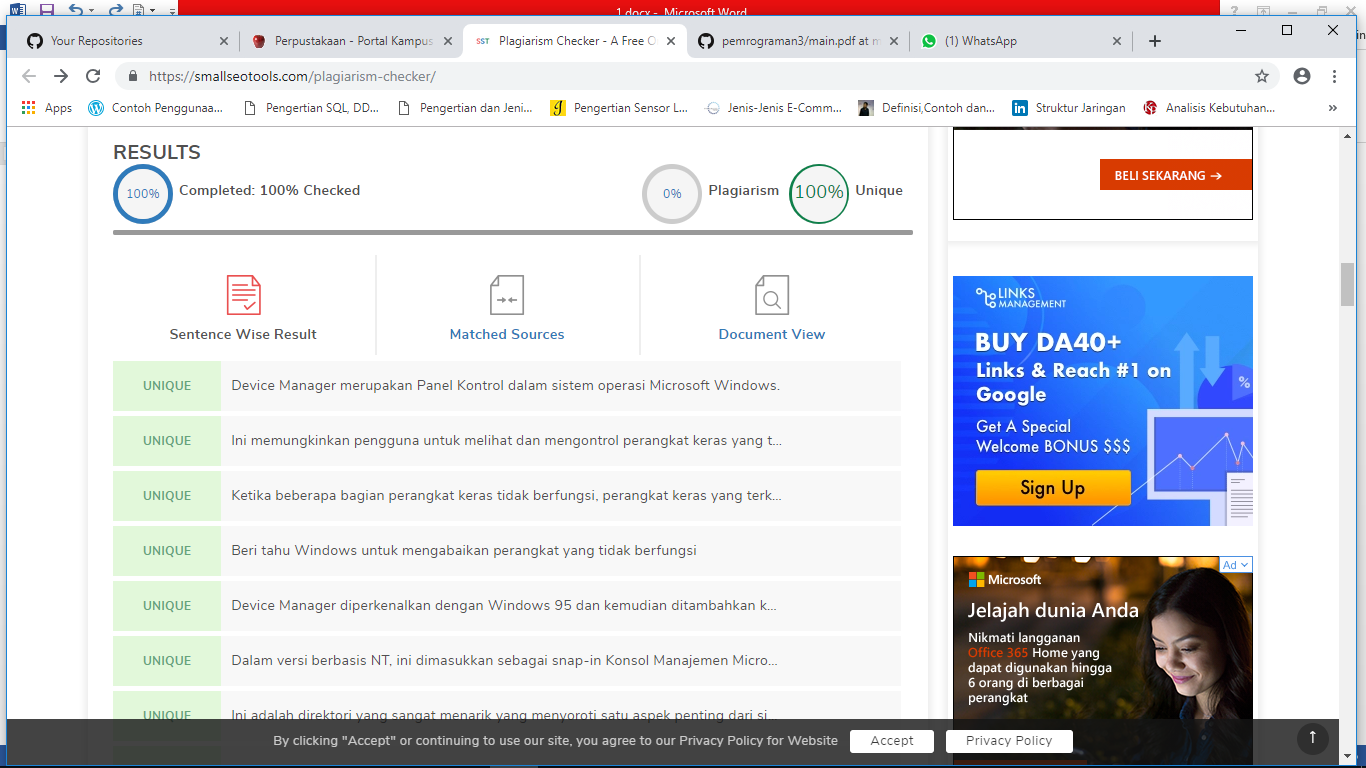
\includegraphics[scale=0.2]{figures/5/1174012/SS2.png}
\caption{plagiarisme}
\label{fig:plagiat}
\end{figure}

%%%%%%%%%%%%%%%%%%%%%%%%%%%%%%%%%%%%%%%%%%%%%%%%%%%%%%%%%%%%%%%%%%%%%%%%%%%%%%%%%%%%%

\section{Dwi Septiani Tsaniyah}
{\Large \textbf{Pemahaman Teori}}
\subsection{Soal No. 1}

Apa itu fungsi device manager di windows dan folder /dev di linux?

\hfill \break
Fungsi device manager dan folder /dev itu berfungsi untuk mengetahui device apa saja yang telah terinstal di leptop anda serta mengetahui port yang digunakan oleh device tersebut.

\hfill \break
Fungsi device manager antara lain :
\begin{enumerate}
	\item Menunjukkan status mengenai suatu perangkat keras.
	\item Menunjukkan informasi detail mengenai suatu perangkat keras.
	\item Mengelola driver perangkat keras.
	\item Menonaktifkan dan mengaktifkan perangkat keras.
	\item Mengidentifikasi konflik antar perangkat keras.
	\item Memberitahukan terjadinya masalah pada perangkat keras.
\end{enumerate}

\subsection{Soal No. 2}
Jelaskan langkah-langkah instalasi driver dari arduino!

\subsection{Jelaskan langkah-langkah instalasi driver dari arduino}
\begin{enumerate}
    \item Cara Auto
    \begin{itemize}
        \item Pertama Hubungkan sistem minimum Arduino Uno ke komputer dengan kabel USB type B(kabel Printer)
        \begin{figure}[H]	
            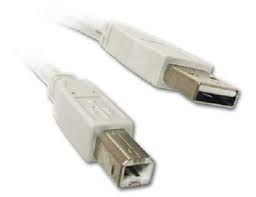
\includegraphics[width=5cm]{figures/5/1174003/teori/kabel.jpg}
            \centering
            \caption{Membuat file csv}
        \end{figure}

        \item Lalu pada bagian kanan didesktop PC anda, akan muncul popup “Installing device driver software” seperti pada gambar dibawah ini.
        \begin{figure}[H]	
            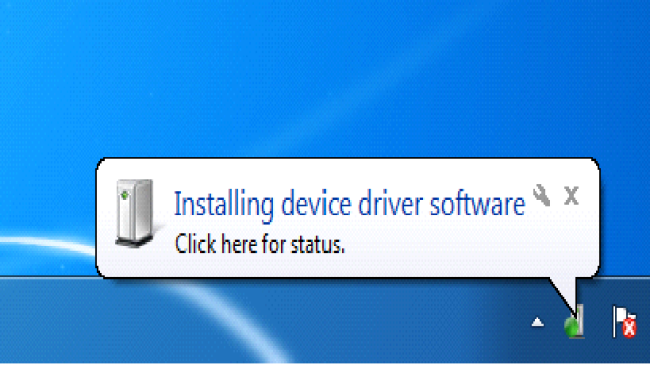
\includegraphics[width=5cm]{figures/5/1174003/teori/1.png}
            \centering
            \caption{Membuat file csv}
        \end{figure}

        \item Tunggu hingga selesai.
        \item Jika sudah selesai anda bisa mengecheck di device manager.
        \begin{figure}[H]	
            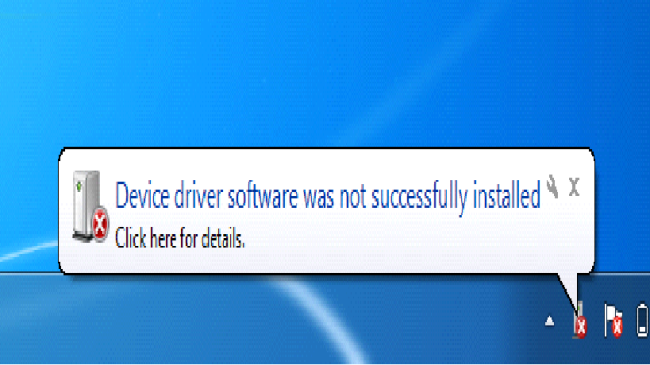
\includegraphics[width=5cm]{figures/5/1174003/teori/2.png}
            \centering
            \caption{Membuat file csv}
        \end{figure}
    \end{itemize}

    \item Cara Manual

    \begin{itemize}
        \item Penginstalan secara manual akan dilakukan jika penginstalan secara auto gagal dilakukan.
        \item Buka Device Manager, caranya pada bagian Search Program and Files lalu ketikkan “device manager”, perhatikan gambar dibawah ini. Pada bagian Control Panel akan muncul Device Manager, klik untuk menjalankan.
            \begin{figure}[H]	
                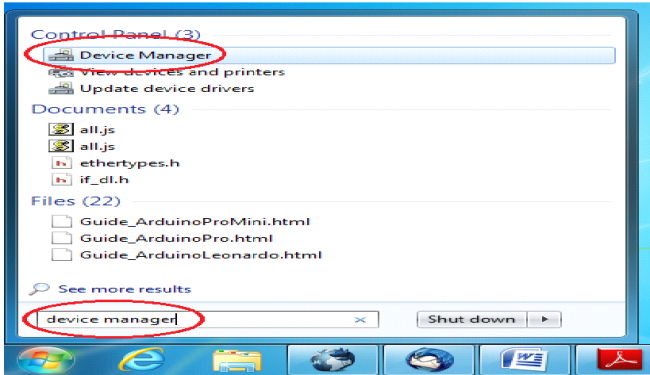
\includegraphics[width=5cm]{figures/5/1174003/teori/3.png}
                \centering
                \caption{Membuat file csv}
            \end{figure}

        \item Cari Unknown device pada bagian Other device, biasanya terdapat tanda seru berwarna kuning, itu disebabkan karena penginstallan tidak berjalan dengan sempurna.
        \begin{figure}[H]	
            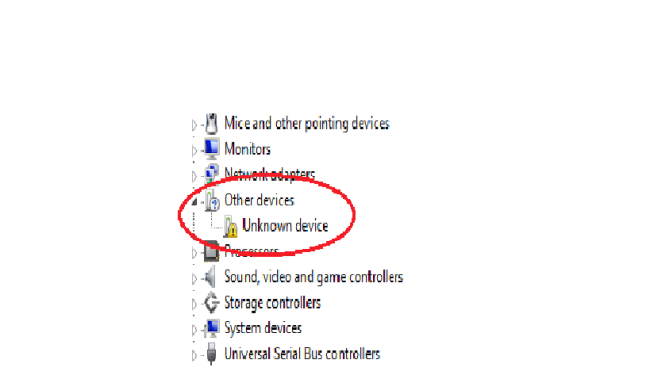
\includegraphics[width=5cm]{figures/5/1174003/teori/4.png}
            \centering
            \caption{Membuat file csv}
        \end{figure}

        \item Klik kanan pada “Unknown device” kemudian pilih Update Driver Software.
        \begin{figure}[H]	
            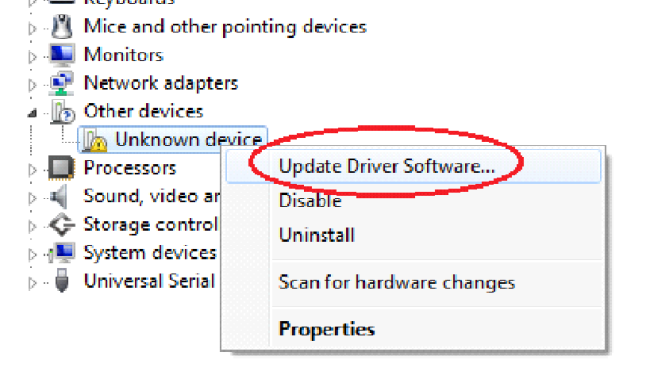
\includegraphics[width=5cm]{figures/5/1174003/teori/5.png}
            \centering
            \caption{Membuat file csv}
        \end{figure}

        \item Pilih Browse my computer for driver software.
        \begin{figure}[H]	
            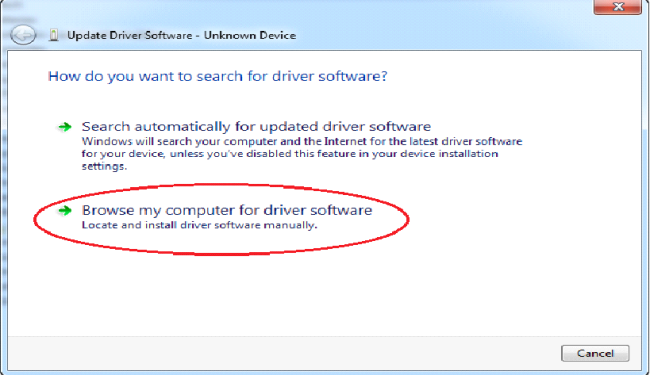
\includegraphics[width=5cm]{figures/5/1174003/teori/6.png}
            \centering
            \caption{Membuat file csv}
        \end{figure}

        \item Arahkan lokasi folder ke folder ..arduino-1.0.5 drivers. Pastikan check-box lalu centang include subfolders. Klik Next untuk melanjutkan instalasi driver.
        \begin{figure}[H]	
            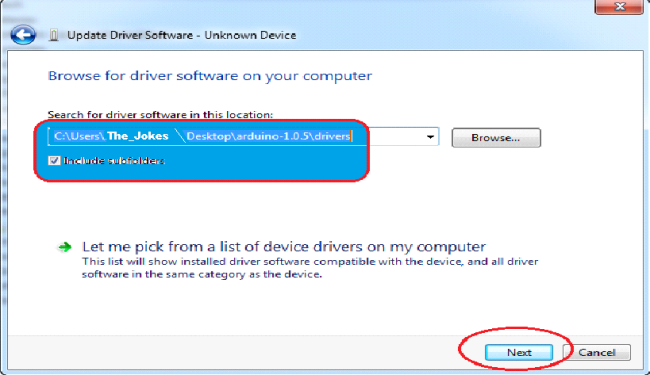
\includegraphics[width=5cm]{figures/5/1174003/teori/7.png}
            \centering
            \caption{Membuat file csv}
        \end{figure}

        \item Kemudian lanjutkan dengan mengklik Install pada tampilan Windows Security.
        \begin{figure}[H]	
            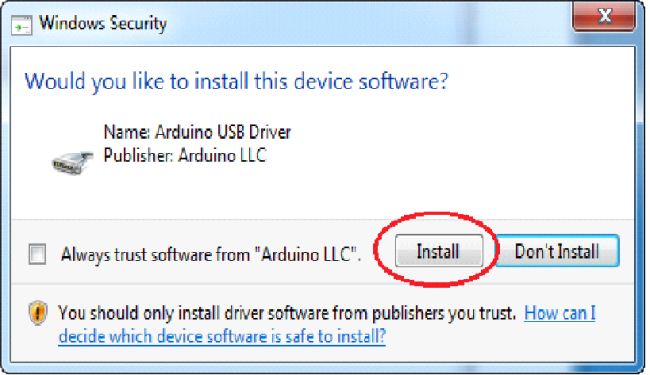
\includegraphics[width=5cm]{figures/5/1174003/teori/8.png}
            \centering
            \caption{Membuat file csv}
        \end{figure}

        \item Jika instalasi driver berhasil maka akan muncul Windows has successfully updated your driver software.
        \begin{figure}[H]	
            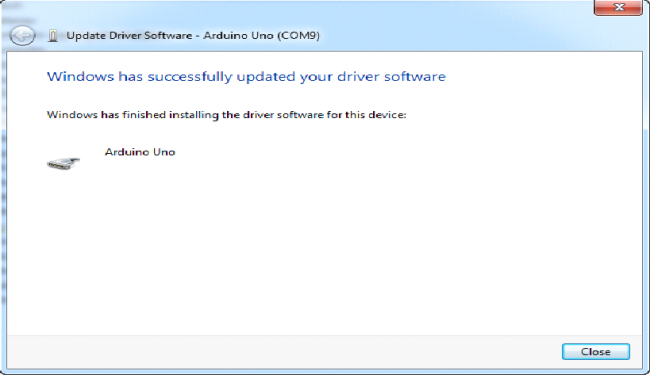
\includegraphics[width=5cm]{figures/5/1174003/teori/9.png}
            \centering
            \caption{Membuat file csv}
        \end{figure}

        \item Perhatikan dan ingat nama COM Arduino Uno, karena nama COM ini yang akan digunakan untuk meng-upload program nantinya.
        \begin{figure}[H]	
            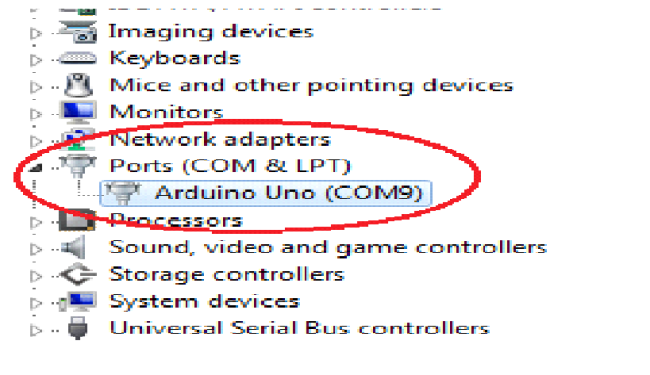
\includegraphics[width=5cm]{figures/5/1174003/teori/10.png}
            \centering
            \caption{Membuat file csv}
        \end{figure}
        \end{itemize}
\end{enumerate}

\subsection{Soal No. 3}
Jelaskan bagaimana cara membaca baudrate dan port dari komputer yang sudah terinstall driver!

Untuk baudrate itu bisa dicek melalui arduino IDE, kemudian untuk mengecheck port bisa dilakukan dengan device manager

\subsection{Soal No. 4}
Jelaskan sejarah library pyserial!

Modul ini merangkum akses untuk port serial. Ini menyediakan backends untuk Python yang berjalan di Windows, Linux, BSD (mungkin sistem yang mendukung POSIX), Jython dan IronPython (.NET dan Mono). Modul bernama "serial" secara otomatis memilih backend yang sesuai. Antarmuka berbasis kelas yang sama pada semua platform yang didukung.

\subsection{Soal No. 5}
Jelaskan fungsi-fungsi apa saja yang dipakai dari library pyserial!

Fungsi-fungsi yang dipakai dari library PySerial, yaitu:
\begin{enumerate}
	\item Serial - fungsi ini untuk membuka port serial.
	\item write(data) - fungsi ini menulis data lewat port serial.
	\item readline() - fungsi ini membaca sebuah string dari port serial.
	\item read(size) - fungsi ini untuk membaca jumlah byte dari port serial.
	\item close() - fungsi ini untuk menutup port serial.
\end{enumerate}

\subsection{Soal No. 6}
Jelaskan kenapa butuh perulangan dan tidak butuh perulangan dalam membaca serial!
\begin{itemize}
\item Perulangan for disebut counted loop (perulangan yang terhitung), sementara perulangan while disebut uncounted loop (perulangan yang tak terhitung). Perbedaannya adalah perulangan for biasanya digunakan untuk mengulangi kode yang sudah diketahui banyak perulangannya. Sementara while untuk perulangan yang memiliki syarat dan tidak tentu berapa banyak perulangannya.
\end{itemize}
\subsection{Soal No. 7}
Jelaskan bagaimana cara membuat fungsi yang mengunakan pyserial!

\subsection{Jelaskan bagaimana cara membuat fungsi yang mengunakan pyserial}
Berikut merupakan contoh penggunaan fungsi yang menggunakan pyserial
\lstinputlisting[firstline=8, lastline=15]{src/5/1174003/T1174003.py}

